\documentclass[tikz]{standalone}

\usepackage[T1]{fontenc}
\usepackage[english]{babel}

\usepackage{standalone}

\usepackage{tikz}

\begin{document}
	\tikzset{
		legend/.style={
			inner sep=0pt,
			text width=7.5cm,
			align=center
		}
	}
	\begin{tikzpicture}
		\node (proj) at (0, 0) {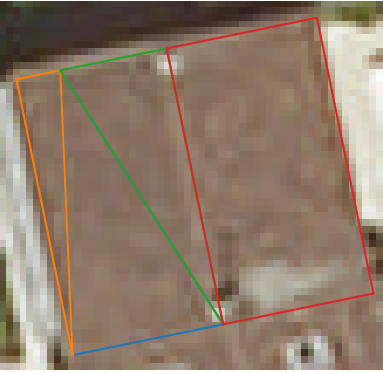
\includegraphics[height=5cm]{images/radio_vector}};
		\path (proj.south) + (0, -2em) node[legend] (proj_legend) {(a) Building nadir projection on an orthoimage.};
		\path (proj.east) + (5, 0) node (grad_edge) {\includestandalone[mode=buildnew, height=5cm]{gradient_edge}};
		\path (grad_edge |- proj_legend.north) node[legend, anchor=north] (grad_edge_legend) {(b) Cosine \underline{similarity} between facet edge normal \textcolor{blue}{$\vec n$} and image gradient \textcolor{purple}{$\vec \nabla I$} for each \textcolor{green}{intersecting} pixel.};
	\end{tikzpicture}
\end{document}
